\documentclass[]{article}
\usepackage{geometry}                           % See geometry.pdf to learn the layout options. There are lots.
\geometry{letterpaper}                                  % ... or a4paper or a5paper or ... 
%\usepackage[parfill]{parskip}                  % Activate to begin paragraphs with an empty line rather than an indent
\usepackage{graphicx}                           % Use pdf, png, jpg, or eps§ with pdflatex; use eps in DVI mode
                                                                % TeX will automatically convert eps --> pdf in pdflatex                
\usepackage{amssymb}
\usepackage{upquote}

%-----------------------------------------------------------------------------
% Special-purpose color definitions (dark enough to print OK in black and white)
\usepackage{color}
% A few colors to replace the defaults for certain link types
\definecolor{orange}{cmyk}{0,0.4,0.8,0.2}
\definecolor{darkorange}{rgb}{.71,0.21,0.01}
\definecolor{darkgreen}{rgb}{.12,.54,.11}
%-----------------------------------------------------------------------------
% The hyperref package gives us a pdf with properly built
% internal navigation ('pdf bookmarks' for the table of contents,
% internal cross-reference links, web links for URLs, etc.)
\usepackage{hyperref}
\hypersetup{pdftex, % needed for pdflatex
  breaklinks=true, % so long urls are correctly broken across lines
  colorlinks=true,
  urlcolor=blue,
  linkcolor=darkorange,
  citecolor=darkgreen,
}

%-----------------------------------------------------------------------------
%
% Commands for annotating the docs with fixme and inter-author notes.  See
% below for how to disable these.
%
% Define a \fixme command to mark visually things needing fixing in the draft,
% as well as similar commands for each author to leave initialed special
% comments in the document.
%% FIXME:  For final printing or to simply disable these bright warnings, copy
%% (there's a target macros_off' in the makefile that does this) the file
%% macros_off.tex to macros.tex

\newcommand{\fix}[1] { \textcolor{red} {
{\fbox{ {\bf Fix:} \ensuremath{\blacktriangleright }} {\bf #1}
\fbox{\ensuremath{\blacktriangleleft} } } } }

% And similarly, one (less jarring, with fewer symbols and no boldface) command
% for each one of us to leave comments in the main text.
\newcommand{\philip}[1] { \textcolor{blue} {
\ensuremath{\blacklozenge} {\bf philip:}  {#1}
\ensuremath{\blacklozenge} } }

\newcommand{\jarrod}[1] { \textcolor{darkgreen} {
\ensuremath{\bigstar} {\bf jarrod:}  {#1}
\ensuremath{\bigstar} } }

\newcommand{\mref}[1] { \textcolor{darkorange} {
\ensuremath{\blacksquare} {\bf missing ref:}  {#1}
\ensuremath{\blacksquare} } }

%% Uncomment these to turn all the special marker commands off
%\renewcommand{\fix}[1]{}
%\renewcommand{\philip}[1]{}
%\renewcommand{\jarrod}[1]{}
%\renewcommand{\mref}[1]{}


\date{}

\begin{document}

\title{Reproducible Applied Statistics:\\
Is tagging of therapist-patient interactions reliable?\thanks{Submitted
to \url{https://github.com/BIDS/repro-case-studies}.
}}

\author{K. Jarrod Millman (JM)\\ Division of Biostatistics\\ UC Berkeley \and
Kellie Ottoboni (KO)\\ Department of Statistics\\ UC Berkeley \and
Naomi A. P. Stark (NS)\\ Department of Philosophy\\ University of Pennsylvania \and
Philip B. Stark (PS)\\ Department of Statistics\\ UC Berkeley
}


\maketitle


\section{Introduction}

This case study illustrates some of the reproducible practices we (JM, KO, PS)
have adopted when working with scientific or domain experts as applied
statisticians.  Parts of the text have been adapted from
\cite{millman2015thesis}.

\begin{enumerate}
\def\labelenumi{\arabic{enumi})}
\itemsep1pt\parskip0pt\parsep0pt
\item
  Who are you and what is your research field?
\end{enumerate}

%\begin{itemize}
%\item
%  K. Jarrod Millman, Division of Biostatistics, UC Berkeley PhD student
%  in biostatistics; background in scientific computing and neuroscience
%\item
%  Kellie Ottoboni, Department of Statistics, UC Berkeley PhD student in
%  statistics
%\item
%  Naomi A.P. Stark, Department of Philosophy, University of Pennsylvania
%  Undergraduate in bioethics; background in therapy with children on the
%  autistic spectrum
%\item
%  Philip B. Stark, Department of Statistics, UC Berkeley Faculty in
%  statistics; background in physical science
%\end{itemize}

We are three applied statisticians~(JM,~KO,~PS) at Berkeley working with a
domain specialist~(NP) at the University of Pennsylvania. Our case study
involves assessing inter-rater reliability (IRR) for human classifiers of
therapy sessions with children on the autistic spectrum.

\begin{enumerate}
\def\labelenumi{\arabic{enumi})}
\setcounter{enumi}{1}
\itemsep1pt\parskip0pt\parsep0pt
\item
  Define what the term ``reproducibility'' means to you generally and/or
  in the particular context of your case study.
\end{enumerate}

The term \emph{reproducibility} is overloaded with orthogonal or even
contradictory meanings in different disciplines. In the context of the current
project, \emph{reproducibility} means that we have documented (nearly) every
step of the analysis, from cleaning to coding to code execution. Of course, the
project itself is \emph{about} the \emph{reliability and replicability} of a
particular kind of measurement: raters' assessments of activities during
therapy sessions.

\section{Workflow narrative}\label{workflow-narrative}

Over the 2014-2015 winter break, NS posed PS a question that came up in her
work on therapeutic interventions with children on the autism scale.
After coming to an intial understanding of her statistical problem,
PS sent JM and KO a one page proposal for a stratified permutation test for
multi-rater inter-rater reliability.

After spending time to understand her underlying research problem and making
certain we understood how her data was collected, we cleaned the data,
developed a nonparametric approach to assessing IRR appropriate to the
experiment, implemented the approach in Python, incorporated the resulting
code into an evolving Python package of permutation
tests (\texttt{permute}\footnote{\url{http://statlab.github.io/permute/}}),
applied the approach to the cleaned data, documented the code and the analysis,
and wrote up the results in a \LaTeX document. 

We distinguish the following aspects of our work:
(1) understand problem,
(2) get and clean data,
(3) design algorithm,
(4) implement algorithm,
(5) analyze data, and
(6) understand result.
In Figure~\ref{fig:work_process}, we've diagrammed an estimate of how much time
we collectively spent on each aspect of the project as well as how each aspect
of the project influenced the other aspects.

\begin{figure}[h]
  \centering
    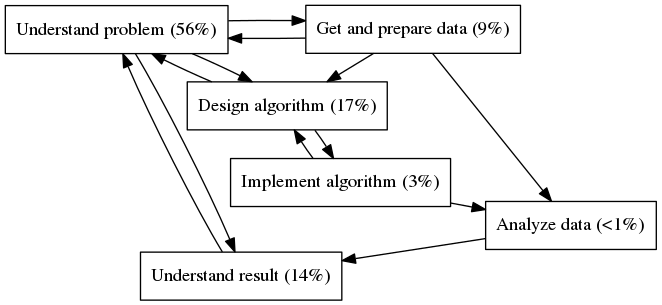
\includegraphics[width=0.8\textwidth]{work_process.png}
  \caption{
  \small
    Each box corresponds to one aspect of our project.
    The percents are estimates of the percent of our time spent on each aspect.
    Edges represent influence. \texttt{Understand problem}~$\to$~\texttt{Design algorithm}
    corresponds to the fact that we first had to understand the problem
    in order to design the correct statistical test.\label{fig:work_process}}
\end{figure}

Underlying all aspects is a set of computational practices
we (JM, KO, PS) followed (almost) whenever we were working on the project.
These computational practices are described in detail
here \cite{millman2014developing} and are used widely
in the open source scientific Python community.
Following these practices, we've developed a Python package for permutation
tests and confidence sets called \texttt{permute}.
We will illustrate how we leverage the software infrastructure of
\texttt{permute} to conduct reproducible and collaborative
applied statistics research with our scientific collaborators.
We discuss the software tools and practices briefly in \S~\ref{key-tools} below.

\subsection{Understand problem (80 hours)}

\philip{
NP was interested in:  What happens in therapy session with autistic kids?
In particular, NP had data and wanted to know whether humans can reliably rate
therapist-patient interactions?
conversations between NS and (primarily) PS to understand the experimental
set-up.
%Time: approximately 10 1-hour meetings
}

\jarrod{
met regularly (approximately weekly, sometimes more) as a team to discuss the
project, work on whiteboards, and use pair programming (JM, KO, PS)
%Time: approximately 10 2-hour meetings.
}

\subsection{Get and clean data (13 hours)}

The data were collected by Naomi Stark and Gil Kliman.
They comprise ratings of segments of 8 videos by 10 trained raters.
Each video is divided into approximately 40 time segments.
In each time segment, none, any, or all of 183 types of activity might be
taking place.
The raters indicated which of those activities was taking place during each
segment of each video.

\philip{
receipt of preliminary data as an Excel spreadsheet; understanding the ``data
dictionary''; vetting for obvious errors (PS);
%Time: approximately 1 hour
several ``trips to the well'' before getting a version of the data that did not
have obvious errors (PS);
%Time: approximately 4 hours
export the Excel data to .csv format (PS);
%Time: approximately 5 minutes.
data anonymization: substitute unique numerical identifiers for raters' names. 
This step was performed using regular expressions in an interactive text
editor, on the .csv file.
It was not performed reproducibly (i.e., not scripted), but it can be checked
readily. (PS) 
%Time: approximately 1 hour.
}

\jarrod{
screen the anonymized data for transcription errors, typos, etc. (JM, PS);
%Time: approximately 5 hours
develop sed scripts to ``correct'' the data for duplicated entries and inferred
typos (JM);
%Time: included above
send cleaned data to NS to verify that the corrections were appropriate (PS, NS);
%Time: 1 hour
include cleaned data in git repo: the anonymized data are public, pre- and
post-cleaning
}

\subsection{Design algorithm (25 hours)}

\jarrod{
``Problem appreciation'': conversations culminating in the decision to assess
the reliability one category at a time. (JM, KO, PS);
%Time: approximately 4h.
Developed an understanding that it was best to treat the videos separately;
Searched the literature for extant approaches to assessing IRR.
We determined that there was no suitable method, in part because the experiment
was stratified and in part because standard methods make indefensible
parametric assumptions, which we hoped to avoid (PS);
%Time: 3h
Decided to use permutation tests;
Decided what the appropriate permutation would be: permuting each rater's
ratings within a video, independently across raters and across videos.
Chose a test statistic to use within each stratum: concordance of ratings;
Derived a simple expression for computing the concordance efficiently (JM, PS);
%Time: 1h
Decided how to combine tests across strata: nonparametric combination of tests,
NPC (JM, KO, PS);
%Time: 1h
Developed a computationally efficient approach to finding the overall p-value
for NPC (JM, KO, PS)
%Time: 1.5h
}

\subsection{Implementing the algorithm (5 hours)}

\jarrod{Fill in.}
  
\subsection{Analyze data (1 hour)}

By the time we got to this stage, the analysis of the cleaned data was only
about 70 lines of Python, of which 56 are code (the rest are comments).
This includes looping over the 183 categories of activity.

\subsection{Understand result (20 hours)}

\philip{We need a discussion of our final thoughts about the data
and how it did or did not address the question.  Maybe a sentence
or two saying what we learned...what we do differently during
data collection next time.
Understanding result can lead to
1) designing new experiment,
2) collecting new data,
3) performing different analysis,
4) writing manuscript,
5) something else. 
}

\section{Pain points}\label{pain-points}

%\emph{Describe in detail the steps of a reproducible workflow which you
%consider to be particularly painful. How do you handle these? How do you
%avoid them? (200-400 words)}

\jarrod{Need to think what is painful here a bit more. A big part of 
why I use the tools I use is to avoid the pain caused by not using
them.  The hand-entered data is a good start.  I think the next
two items need to be rewritten some.  The pain being, I would argue,
that most of didn't already know these tools well.} 

Vetting hand-entered data; ensuring that the data are relatively
error-free.

Learning and setting up new workflow tools, such as TravisCI.

Maintaining coding and naming conventions.

\section{Key benefits}\label{key-benefits}

%\emph{Discuss one or several sections of your workflow that you feel
%makes your approach better than the ``normal'' non-reproducible workflow
%that others might use in your field. What does your workflow do better
%than the one used by your lesser-skilled colleagues and students, and
%why? What would you want them to learn from your example? (200-400
%words)}

\jarrod{confidence?  you much we trust and stand behind our work.
how likely would I be to build off the work.}

It's easy to modify the analysis if errors are found, to apply the
analysis to new data sets, and so on.

The process is largely self-documenting, making it easier to draft a
paper about the results.

The methods are abstracted from the analysis and incorporated into a
package so that others can discover, check, use, and extend the
methods.

\section{Key tools and practices}\label{key-tools}

%\emph{If applicable, provide a detailed description of a particular
%specialized tool that plays a key role in making your workflow
%reproducible, if you think that the tool might be of broader interest or
%relevance to a general audience. (200-400 words)}

As part of the development of our software package \texttt{permute}, we
invested significant effort in setting up a development infrastructure to
ensure our work is tracked, thoroughly and continually tested, and
incrementally improved and documented.
To this end, we have adopted best practices for software development used by
many successful open source projects \cite{millman2014developing}.

\subsection{\label{sec:vc}Version control and code review}

We use Git\footnote{\url{http://git-scm.com}} as our version control system
(VCS) and GitHub\footnote{\url{https://github.com}} as the public hosting
service for our official \texttt{upstream} repository
(\url{https://github.com/statlab/permute}).
Each developer has their own copy, or fork, of the \texttt{upstream}
repository.
We each work on our own repositories and use the \texttt{upstream} repository
as our coordination or integration repository.

Git allows us to track and manage how our code changes over time as well as
review all new functionality before merging it into the \texttt{upstream}
repository.
To get new code integrated in the \texttt{upstream} repository, we use GitHub's
\emph{pull request} mechanism.
This enables us to review code before integrating it.
Below, we describe how we automate our testing to generate reports for all pull
requests.
This way we can reduce the risk that changes to our code break existing
functionality.
Once a pull request is reviewed and accepted, it is merged into the
\texttt{upstream} repository.

Requiring all new code to undergo review provides several benefits.
Code review increases the quality and consistency of our codebase.
It helps maintain a high level of test coverage (see below).
Moreover, it also helps keep the development team aware of the work other team
members are doing.
While we are currently a small team and we meet regularly, having the code
review system in place will make it easier for new people to contribute as well
as capturing our design discussions and decisions for future reference.

\subsection{\label{sec:test}Testing and continuous integration}

We use the \texttt{nose} testing framework for automating our testing
procedures.\footnote{\url{https://nose.readthedocs.org}}
This is the standard testing framework used by the core packages in the
scientific Python ecosystem.
Automating the tests allows us to monitor a proxy for code correctness when
making changes as well as simplifying the code review process for new code.
Without automated testing, we would have to manually test all the code every
time a change is proposed.
The \texttt{nose} testing framework simplifies test creation, discovery, and
running.
It has an extensive set of plugins to add functionality for coverage reporting,
test annotation, profiling, as well as inspecting and testing documentation.

\begin{figure}
  \begin{centering}
    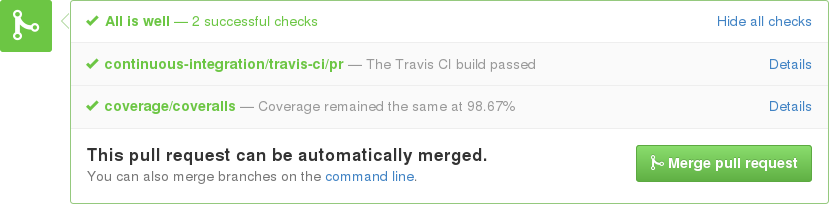
\includegraphics[width=\textwidth]{pull-request-ci.png}\par
  \end{centering}

  \caption{\label{fig:pull-request}
  \small
    Each pull request triggers an automated system to run the  full test suite on
    the updated codebase.
    This means that when you go to review a pull request you can immediately see
    whether the change breaks any of the tests as well as whether the new
    code decreases the overall test coverage.
    For example, the above report indicates that the associated pull request does not
    break existing code and does not change our test coverage.}
\end{figure}

Our goal is to test every line of code.
For example, not only do we want to test every function in our package, but if
a specific function has internal logic we want to test each possible execution
path through the function.
Having tested each line of code increases our confidence in our codebase, but
more importantly provides us some measure of assurance that changes we make do
not break existing code.
It also increases our confidence that new code works, which reduces the
friction of accepting contributions.
Currently over 98\% of \texttt{permute}'s lines of code get executed at least
once by our test system.

We have configured Travis CI\footnote{\url{https://travis-ci.org}} and
\texttt{coveralls}\footnote{\url{https://coveralls.io}} to be automatically
triggered whenever a commit is made to a pull request or the upstream master
(see Figure~\ref{fig:pull-request}).
These systems then run the full test suite  using different versions of our
dependencies (e.g., Python 2.7 and 3.4) every time a new commit is made to a
repository or pull request.

\subsection{\label{sec:doc}Documentation}

We use Sphinx\footnote{\url{http://sphinx-doc.org}} as our documentation system
and already have good developer documentation and the foundation for
high-quality user documentation.
Sphinx is the standard documentation system for Python projects and is used by
the core scientific Python packages.
We use Python docstrings and follow the NumPy docstring
standard\footnote{\url{https://github.com/numpy/numpy/blob/master/doc/HOWTO\_DOCUMENT.rst.txt}}
to document all the modules and functions in \texttt{permute}.
Using Sphinx and some NumPy extensions, we have a system for autogenerating the
project documentation (as HTML or PDF) using the docstrings as well as
stand-alone text written in a light-weight markdown-like language, called
reStructuredText\footnote{\url{http://docutils.sourceforge.net/rst.html}}.
This system enables us to easily embed references, figures, code that is
auto-run during documentation generation, as well as mathematics using \LaTeX.

\subsection{\label{sec:release}Release management}

Our development workflow ensures that the official \texttt{upstream} repository
is always stable and ready for use.
This means anyone can get our official upstream master at any point, install it
and start using it.
We also make official releases available as source tarballs as well as Python
built-packages\footnote{Presently our code is pure Python, but we release
Python wheels.
Wheels are the new standard built-package format for Python.} uploaded to the
Python Package Index, or PyPI,\footnote{PyPI is the Python equivalent of \emph{The
Comprehensive R Archive Network} (CRAN).} with release announcements posted to
our mailing list.

To install the latest release of \texttt{permute} and its dependencies, type
the following command from a shell prompt (assuming you have Python and a
recent version of pip):

\texttt{\$ pip install permute}


%\textbf{Software tools:}
%
%    \begin{enumerate}
%    \def\labelenumiii{\alph{enumiii}.}
%    \itemsep1pt\parskip0pt\parsep0pt
%    \item
%      \emph{virtualenv} to control which versions of which software
%      packages were used. \emph{virtualenv} is a tool to create isolated
%      Python environments.
%    \item
%      \emph{git} for revision control
%    \item
%      \emph{github} for hosting
%    \item
%      \emph{make} for process automation
%    \item
%      \emph{nose} to automate and document testing
%    \item
%      \emph{sphinx} for documentation in HTML and PDF
%    \item
%      \emph{Python} as the language for data analysis
%    \item
%      \emph{Github} pull requests to control code review.
%    \item
%      \emph{TravisCI} and \emph{BuildBot} for continuous integration
%      during code development
%    \item
%      \emph{Coverage/Coveralls} to check the code coverage of the
%      \emph{nose} tests
%    \item
%      \emph{PyPI} to distribute built packages
%    \item
%      LaTeX for documents, especially documents containing mathematical
%      notation
%    \end{enumerate}
%    
%\textbf{Coding practices.}
%
%    \begin{enumerate}
%    \def\labelenumiii{\alph{enumiii}.}
%    \itemsep1pt\parskip0pt\parsep0pt
%    \item
%      Tests for all code; Coverage/Coveralls to check test coverage.
%    \item
%      Pair programming, at least some of the time
%    \item
%      Issue trackers in git
%    \item
%      All code vetted using pull requests: no pushes. Circular flow of
%      code from main repo to individual repos to main repo.
%    \item
%      Use whiteboard to sketch algorithms before coding
%    \item
%      Documentation: internal to the code, external in the Github repo
%      and github.io; external in the package
%    \item
%      Test data included with the package
%    \end{enumerate}


\bibliographystyle{plain}
\bibliography{millman_ottoboni_stark}

\end{document}
